\section{Csavarkötések}%###############################################################

\subsection{Előfeszítő erő meghatározása}%============================================================
\label{csavarkotes}

\begin{wrapfigure}{r}{.4\textwidth}
 \vspace{-2cm}
 \centering
 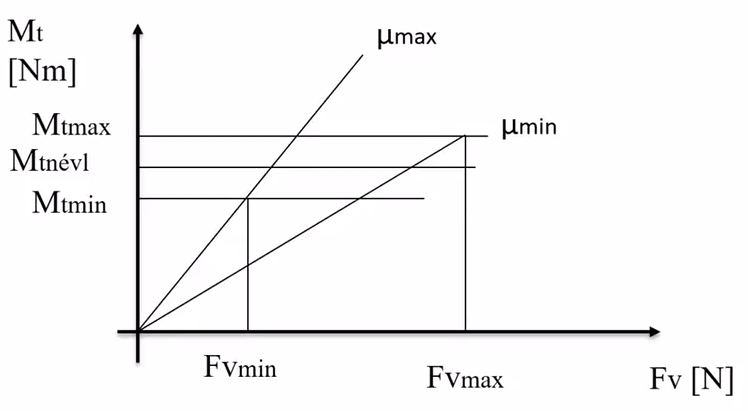
\includegraphics[width=\linewidth]{klein}
 \caption{Klein-diagram}
\end{wrapfigure}
\parbox{.55\textwidth}{
\begin{outline}
	\1 adatok
		\2 M10, metrikus anyát nyomatékkulcsal húzunk meg
		\2 előírt meghúzási nyomaték 35 Nm
		\2 nyomatékkulcs hibája $\pm 5\%$
		\2 a súrlódási tényező $\mu\in[0.08, 0.12]$
		\2 a menet magátmérője 7.19 mm, közepes átmérője 9.03 mm, menetemelkedése 1.5 mm
		\2 az anya laptávolsága 16 mm
		\2 az átmenő furat átmérője 11 mm
		\2 Mekkora az előfeszítő erő minimális és maximális értéke?\vspace{3mm}
\end{outline}}
\begin{outline}
	\1 megoldás
		\2 $M_\text{t} = M_\text{v} + M_\text{a}$
		\2 meneteken ébredő súrlódásból eredő nyomaték: $M_\text{v} = F_\text{k}\frac{d_2}{2} = F_\text{v}\tan\brc{\alpha+\rho'}\frac{d_2}{2}$
		\2 homlokfelületen fellépő súrlódásból eredő nyomaték: $M_\text{a} = F_\text{v}\frac{d_a}{2}\mu_\text{a}$
		\2 menetemelkedési szög: $\alpha = \arctan\frac{P}{d_2\pi}$
		\2 látszólagos súrlódási félkúpszög: $\rho' = \arctan\frac{\mu}{\frac{\cos\beta}{2}}$
		\2 $\beta = \case{60^\circ\text{ -- metrikus menet}\\55^\circ\text{ -- Whitworth/csőmenet}\\30^\circ\text{ -- trapézmenet}}$
		\2 $d_\text{a} = \frac{D+s}{2} = 13.5 \text{ mm}$ ( $s$ az anya laptávolsága)
		\2 $\alpha = 3.027^\circ$
		\2 $\rho'_\text{min} = 5.28^\circ$
		\2 csavarkötés akkor önzáró, ha $\rho'>\alpha$
		\2 $F_\text{v min} = 19783$ N
		\2 $F_\text{v max} = 30649$ N
\end{outline}

\subsection{Anya magasság számítása}%============================================================

\begin{wrapfigure}{r}{.4\textwidth}
 \vspace{-4cm}
 \centering
 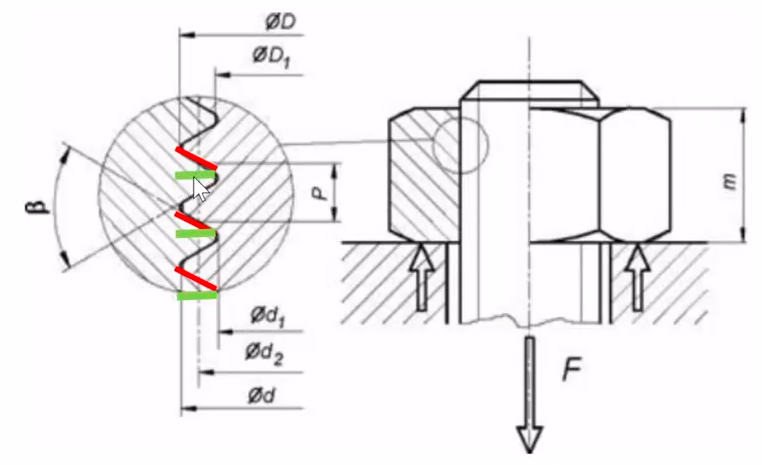
\includegraphics[width=\linewidth]{csavarnyomas}\\
 % \hspace{1cm}
 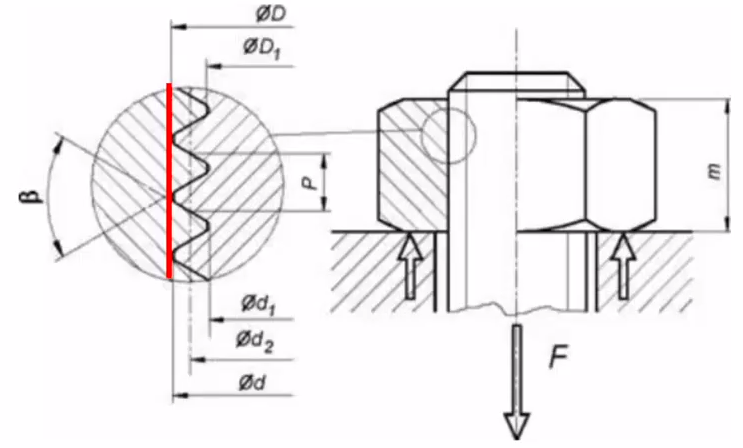
\includegraphics[width=\linewidth]{csavarnyiras}
 \caption{Nyomott és nyírt terület}
\end{wrapfigure}
\parbox{.6\textwidth}{
\begin{outline}
	\1 adatok
		\2 M20-as csavarkötés
		\2 $F_\text{v} = 60000$ N
		\2 a megengedhető felületi nyomás $p_\text{meg} = 80$ MPa
		\2 a maximális csúsztatófeszültség $\tau_\text{meg} = 190$ MPa
		\2 $d_2 = 18.376$ mm, $d_3 = 16.933$ mm, $P = 2.5$ mm
		\2 Mekkora legyen az anya magassága?
	\1 megoldás
		\2 $p = \frac{F}{A_\text{p}} \le p_\text{meg}$
		\2 $A_\text{p} = \brc{\frac{d^2\pi}{4} - \frac{d_3^2\pi}{4}}i = 750 \text{ mm}^2$
		\2 $i_\text{p} = 8.4$ menet
		\2 $A_\tau = d\pi pi$
		\2 $\tau_\text{meg} = \frac{F}{A_\tau}~\rightarrow~A_\tau=315.8\text{ mm}^2$
		\2 $i_\tau = 2$ menet
		\2 $\operatorname{ceil}[\max(i_\text{p}, i_\tau)] = 9$ menet
\end{outline}}

\subsection{Csavar méretezése megnyúlásra}%============================================================

\begin{outline}
	\1 adatok
		\2 M16-os magragyengített csavar
		\2 $L$ hosszon a csavarszár átmérője $d_5$-re csökken
		\2 Mekkora nyomatékkal kell meghúzni hogy a megnyúlás $\Delta L=0.075$ mm-es legyen?
		\2 Mekkora a csavar minimális szakítószilárdsága?
	\1 megoldás
		\2 $\Delta L = \frac{F_\text{v}L}{AE}\rightarrow F_\text{v} = AE\frac{\Delta L}{L}$
		\2 $A = \frac{d_5^2\pi}{4} = 113.1 \text{ mm}^2$
		\2 $F_\text{v} = 18176$ N
		\2 A \ref{csavarkotes}-es alszakasz alapján $M_t = 38844$ Nmm
		\2 $\sigma = \frac{F}{A} = 160.7$ MPa
		\2 $\tau = \frac{M_tau}{I_\text{p}}e = 114.5$ MPa
		\2 itt vagy a tömör ($d_3$), vagy a névleges ($d_2$) átmérővel számolunk
		\2 $\sigma_\text{HMH} = 255.3$ MPa
\end{outline}
